\documentclass[class=article,border=0pt]{standalone}

%------------------------------------------------------------------------------
%                         COLORS
%------------------------------------------------------------------------------
\usepackage{xcolor}

%------------------------------------------------------------------------------
%                          TIKZ
%------------------------------------------------------------------------------
\usepackage{tikz}
\usepackage{pgfplots}
\pgfplotsset{width=10cm,compat=1.15}
\usetikzlibrary{shapes.arrows}

\tikzset{
	graphnode/.style = {align=center, inner sep=0pt, text centered, font=\sffamily},
	kmer/.style = {graphnode, circle, black, font=\sffamily\bfseries, draw=black, fill=white, text width=3em},
}

\definecolor{darkgreen}{rgb}{0.0, 0.65, 0.31}

\begin{document}
	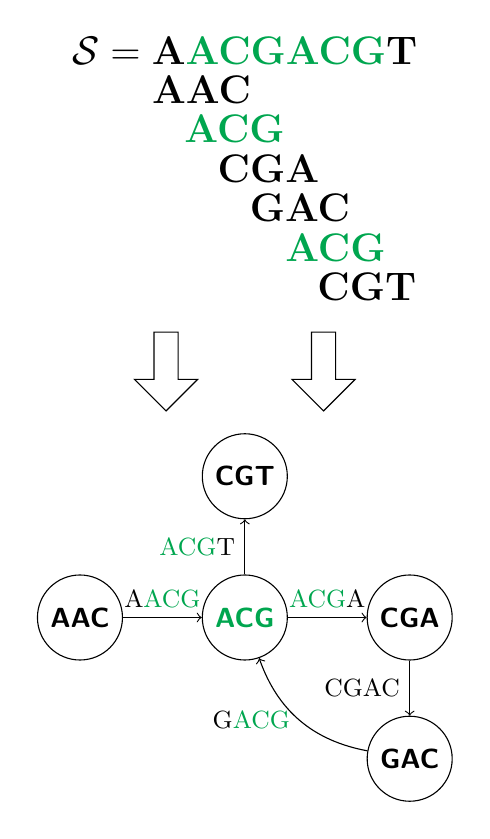
\begin{tikzpicture}	
	%\path (k1) edge[->, line width=1] node[above, rotate=-45]{GACG} (k4);
	%\path (k2) edge[->, line width=1] node[above]{CGAC} (k1);
	%\path (k3) edge[->, line width=1] node[above]{AACG} (k4);
	%\path (k4) edge[->, line width=1] node[above, rotate=45]{ACGA} (k2);
	%\path (k4) edge[->, line width=1] node[above, rotate=-45]{ACGT} (k6);
	%\path (k6) edge[->, line width=1] node[above]{CGTA} (k7);
	%\path (k7) edge[->, line width=1] node[above]{GTAC} (k5);
		
	\node[font=\Large\bfseries] at (0, 4) {$\mathcal{S} = \mathbf{A{\color{darkgreen} ACGACG}T}$};
	\node[font=\Large\bfseries] at (-0.55, 3.5) {$\mathbf{AAC}$};
	\node[font=\Large\bfseries] at (-0.13, 3) {$\color{darkgreen} \mathbf{ACG}$};
	\node[font=\Large\bfseries] at (0.3, 2.5) {$\mathbf{CGA}$};
	\node[font=\Large\bfseries] at (0.7, 2) {$\mathbf{GAC}$};
	\node[font=\Large\bfseries] at (1.15, 1.5) {$\color{darkgreen} \mathbf{ACG}$};
	\node[font=\Large\bfseries] at (1.55, 1) {$\mathbf{CGT}$};
	
	\node[draw, single arrow,
	minimum height=10mm, minimum width=8mm,
	single arrow head extend=2mm, rotate=-90] at (-1,0) {};

	\node[draw, single arrow,
	minimum height=10mm, minimum width=8mm,
	single arrow head extend=2mm, rotate=-90] at (1,0) {};
	
	\matrix[row sep=7mm,column sep=10mm] at (0, -3.2) {
			& \node[kmer](k1){CGT}; & \\
			\node[kmer](k2){AAC}; & \node[kmer](k3){\color{darkgreen} ACG}; & \node[kmer](k4){CGA}; \\
			& & \node[kmer](k5){GAC}; \\
	};

	\path (k2) edge[->] node[above]{\small A{\color{darkgreen} ACG}} (k3);
	\path (k3) edge[->] node[above]{\small {\color{darkgreen} ACG}A} (k4);
	\path (k4) edge[->] node[left]{\small CGAC} (k5);
	\path (k5) edge[->, bend left=30] node[left]{\small G{\color{darkgreen} ACG}} (k3);
	\path (k3) edge[->] node[left]{\small {\color{darkgreen} ACG}T} (k1);
	\end{tikzpicture} 
	
\end{document}